\section{Proposed Improvements to BGP}\label{sec:discussion}

Thus far, this chapter has focused on predicting BGP route selection
inside a single AS.  Notably, two artifacts, the MED attribute and route
reflection, complicate this process.  Not only do these attributes make
route prediction difficult, {\em they also create problems with the
  operation of 
BGP itself}.  The use of MED, both with and without route reflection has
been shown to cause oscillation~\cite{Basu2002}; route reflection can
also prevent convergence and cause forwarding loops~\cite{Griffin2002}.
The MED attribute is intended to allow a neighboring AS to dictate
preferred exit points on routes advertised at multiple exit points, but
it prevents a router from forming a consistent ordering of preferences
over routes.  Route reflectors were introduced to allow an iBGP topology
to scale, but they do so in a way that prevents routers from 
discovering the complete set of eBGP-learned routes.  

In this section, we explore possible solutions to the problems
introduced by MED and route reflection.  A major lesson one should draw
from this section is that a system that had visibility into an AS's
topology, configuration, and available BGP routes could actively {\em
control} the BGP route selection process, rather than simply trying to
predict its outcome.  The Routing Control Platform
(RCP)~\cite{caesar2004,feamster:fdna2004}, whose design we will 
discuss in Chapter~\ref{chap:concl}, can thus not only help
ensure correctness (as discussed briefly in
Section~\ref{sec:rcc_lessons}), but also make Internet routing easier to
control (and, hence, predict).

\subsection{MED-ication for Late-Exit Semantics}\label{sec:sandbox:med_disc}


The MED attribute causes problems because it is not comparable across
routes from different neighboring ASes, which prevents a router from
producing a consistent total ordering over all possible routes.  Also,
in networks without route reflection, inconsistent
preferences between pairs of routes is based on the router ID attribute,
an arbitrary tiebreak that carries no meaningful semantics (as in
Figure~\ref{fig:med}, for example).  

Before we consider solutions to the problems introduced by MED, it is
worth noting that MED, as it operates today and when used with
route reflection {\em may not have the intended effect on route selection}.
Consider the example shown in Figure~\ref{fig:ibgp2}.  A neighboring AS
sending routes $a$ and $b$ with MED values $10$ and $20$, respectively,
expects that the AS shown would always prefer route $a$ over route $b$,
as long as both existed, causing router $X$ to perform late-exit routing
(\ie, send its traffic via route $b$ via router $Y$).  Unfortunately,
the AS shown will {\em not} do so: $RR$ prefers route $c$, so router $X$
will never learn route $b$, and it will continue to forward packets via
route $a$.

We observe that if MED values are {\em remapped} into an explicit
ranking across neighboring ASes, rather than arbitrary values, then the MED
attribute 
{\em can} be compared across all routes at step~4 of the route selection
process (as it is today).  Comparing an exit-rank across
all routes can sometimes result in different outcomes than BGP today,
but in many cases the differences do not affect the important semantics
of BGP.  For example, consider Figure~\ref{fig:med}, but where the MED
attribute is compared across all routes.  Suppose that the route
selection process retains the MED comparison step, but that AS 2's MED
values of $10$ and $20$ are remapped to $1$ and $2$, and that the
highest MED value of any eBGP-learned route, $2$, is added to the MED
value on every route learned via iBGP (this transformation guarantees
that comparing MEDs across all routes would not cause iBGP-learned
routes to be preferred over eBGP-learned routes).  In this case, routers
$X$ and $Y$ would ultimately select routes $c$ and $d$, respectively, as
opposed to $a$ and $d$ in BGP today.  Although $X$ selects $c$ instead
of $a$, its preference between these two routes was based on the
arbitrary router ID tiebreak; therefore, having router $X$ select $c$
instead does not destroy any meaningful semantics.

The type of remapping we have described preserves MED's semantics,
%(as opposed MED's operation today, which provides no such guarantee),
but implementing an exit-rank requires visibility into the set of
available routes that is not available today.  Unfortunately, MED values
are typically based on dynamic values (\eg, IGP path costs across the
network), so an AS that sends routes with MED values cannot simply
configure a static 
ranking.  Given today's architectures, neither the sending nor receiving
AS could perform a remapping of MED values into an exit-rank, since no
single router learns the complete set of routes advertised from a
neighboring AS.  Performing such a remapping would require either the
sending or receiving AS to have complete visibility over all routes
being sent or received for a destination.  On the other hand, the
Routing Control Platform (RCP)~\cite{feamster:fdna2004} or similar
recently proposed architectures~\cite{id-versatile-rr} can perform such
a remapping, since RCP has full visibility of routes sent from a
neighboring AS (as well as full control over the routes that it sends to
a neighboring AS).
%
This modification allow the algorithm from Figure~\ref{fig:b2_tot_order}
to correctly compute 
the outcome of BGP route selection, and it would also eliminate intra-AS
safety problems.


\subsection{Scalability without Route Reflection} 

%% \begin{figure}[t]
%% \centering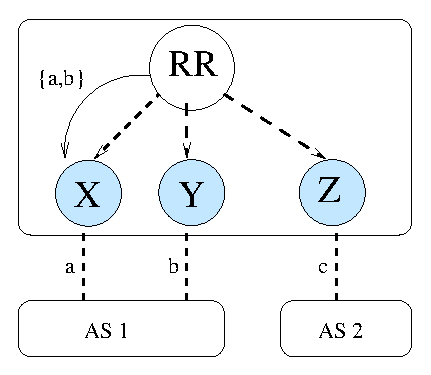
\epsfig{file=sandbox/figures/deflect.eps,width=0.45\linewidth}
%% \caption{Previous solutions~\protect\cite{Basu2002} to the MED
%%   oscillation problem can cause deflections and loops in some cases.  If
%%   $RR$ selects route $b$ but sends both $b$ and $c$ to router $X$, then
%%   $X$ might select route $c$ (\eg, for traffic engineering reasons,
%%   such as offloading traffic to AS 2).  However, packets forwarded from
%%   $X$ to $RR$ will still use $RR$'s best route $b$.}
%% \label{fig:deflect}
%% \end{figure}


Route reflectors allow iBGP topologies to scale to large number of
routers because they obviate the need to have a ``full mesh''
topology with $O(|R|^2)$ sessions. Unfortunately, they restrict route
visibility 
because they only send a single best route from all of the routes they
have learned.  In this chapter, we have explained how this restriction
complicates predicting the outcome of BGP route selection; previous work
has also 
noted that it can cause persistent oscillation and forwarding
loops~\cite{Basu2002, Griffin2002}.   

To remedy the problems with persistent oscillation, Basu {\em et al.}
proposed that route reflectors forward {\em all routes} that are equally
good up to and including the MED comparison.  It turns out that this
modification correctly emulates a full mesh iBGP topology; thus, it is
possible to model the outcome of their modified protocol with the
algorithm from Figure~\ref{fig:b2_no_tot_order}.  
Unfortunately,
this proposal
% has two significant drawbacks.  First, 
requires modifications to the routers, since each router readvertises
multiple routes instead of a single best route.  Additionally, because
each router readvertises multiple routes to its neighboring routers,
every router must select routes using a {\em consistent} selection criterion.
Otherwise, given multiple routes, some router along the path to an egress
router might select a different route, violating route
validity (Definition~\ref{defn:rv}).  This 
restriction precludes certain policies and configurations (\eg, a
router may not manipulate attributes on a route learned via iBGP).

%% Second, having a route
%% reflector advertise multiple routes while forwarding packets only on the
%% locally best route can cause deflections in circumstances where not all
%% routers along the path to an exit router select the same route.
%% Consider Figure~\ref{fig:deflect}.  Suppose $RR$ selects route $b$ and
%% sends routes $b$ and $c$ to router $X$.  Also assume that router $X$
%% prefers route $c$ over route $b$; such a situation could occur, for
%% example, if (1)~a network operator explicitly lowered the local
%% preference of routes from AS $1$ on router $X$ to offload some traffic
%% on that link, or (2)~the router ID tiebreak at router $X$ selects route
%% $c$.  If $X$ prefers $c$ over $b$, but its path to $Z$ traverses $RR$,
%% then $RR$ will forward packets intended for route $c$ via route $b$
%% instead. 

Architectures such as RCP propose separating route selection from the
routers and placing this functionality in a system that computes routes
on behalf of all of the routers within an AS~\cite{feamster:fdna2004}.
Rather than returning only a single best route to all of its clients (as
a route reflector does), RCP advertises to each router {\em the route
that it would have selected in a full mesh iBGP configuration}.  This
architecture allows the network to scale in the same way that route
reflectors do, but it provides some important additional advantages.
First, because RCP explicitly assigns routes to all routers in the
network, it can {\em guarantee} that the route assignments satisfy route
validity.  Second, RCP allows for a more 
scalable network design.  Furthermore, RCP does not have to make the
same routing decisions as its clients (as route reflectors do today).
As a result, unlike route reflectors, RCP nodes can be replicated at
arbitrary places in the IGP topology.

